%%%%%%%%%%%%%%%%%%%%%%%%%%%%%%%%%%%%%%%%%%%%%%%%%%%%%%%%%%%%%%%%%
% MUW Presentation
% LaTeX Template
% Version 1.0 (27/12/2016)
%
% License:
% CC BY-NC-SA 4.0 (http://creativecommons.org/licenses/by-nc-sa/3.0/)
%
% Created by:
% Nicolas Ballarini, CeMSIIS, Medical University of Vienna
% nicoballarini@gmail.com
% http://statistics.msi.meduniwien.ac.at/
%%%%%%%%%%%%%%%%%%%%%%%%%%%%%%%%%%%%%%%%%%%%%%%%%%%%%%%%%%%%%%%%%
\documentclass[8pt,pdf,hyperref={unicode}, xcolor=dvipsnames, fleqn]{beamer}
\usepackage{array} % Для титульника
\usepackage{ucs}
\usepackage[utf8x]{inputenc} % Включаем поддержку UTF8

%%%%XeLaTex part%%%
\usepackage{polyglossia}   %% загружает пакет многоязыковой вёрстки
\setdefaultlanguage{russian}  %% устанавливает главный язык документа
\setotherlanguage{english} %% объявляет второй язык документа
\defaultfontfeatures{Ligatures={TeX}}  %% свойства шрифтов по умолчанию
\setmainfont[Ligatures={TeX,Historic}]{Times New Roman} %% задаёт основной шрифт документа
\setsansfont{Arial}                    %% задаёт шрифт без засечек
\setmonofont{Courier New}               %% задаёт моноширинный шрифт
\newfontfamily{\cyrillicfonttt}{Courier New} % моноширинный шрифт, на который не ругается компилятор

\usetheme{MUW}
\usecolortheme{MUW}
\setbeamertemplate{navigation symbols}{} 
\setbeamertemplate{caption}[numbered]

%%%%%%%%%%%%%%%%%%%Button settings%%%%%%%%%%%%%%%%
%\definecolor{light-gray}{gray}{0.95}
%\setbeamercolor{button}{bg=white,fg=black}

%%%%%%%%%%%%%%%Список литературы
\usepackage[square, numbers, sort&compress]{natbib}
\newcommand{\empline}{\mbox{}\newline}
\renewcommand{\bibnumfmt}[1]{#1.\hfill}
%\renewcommand{\bibsection}{\chapter{ {\LARGE Список литературы}}}

\setlength{\bibsep}{0pt}
%%%%%%%%%%%%%%%Список литературы


%%%%%%%%%%%%%%%%%%%%%%%%%%%%%%%%%%%%%%%%%%%%%%%%%%%%%%%%%%%%%%%%%
%% Presentation Info
\title[Введение в язык программирования Python]{\textit{Занятие 1}: ~\\ Введение в язык программирования Python}
\author{ФКН}
\institute{Воронежский государственный университет}
\date{

	\begin{figure}
		
\includegraphics[height=0.15\textwidth]{Images/python.png}
		%\caption{\label{fig:your-figure}Caption goes here.}
	\end{figure}


			
}
%%%%%%%%%%%%%%%%%%%%%%%%%%%%%%%%%%%%%%%%%%%%%%%%%%%%%%%%%%%%%%%%%


%%%%%%%%%%%%%%%%%%%%%%%%%%%%%%%%%%%%%%%%%%%%%%%%%%%%%%%%%%%%%%%%%
%% FOOTLINE
%% Comment/Uncomment the following blocks to modify the footline
%% content in the body slides. 


%% Option A: Title and institute
%\footlineA
%% Option B: Author and institute
%\footlineB
%% Option C: Title, Author and institute
\footlineC
%%%%%%%%%%%%%%%%%%%%%%%%%%%%%%%%%%%%%%%%%%%%%%%%%%%%%%%%%%%%%%%%%

\begin{document}

%%%%%%%%%%%%%%%%%%%%%%%%%%%%%%%%%%%%%%%%%%%%%%%%%%%%%%%%%%%%%%%%%
% Use this block for a blue title slide with modified footline
{\titlepageBlue
\begin{frame}
  \titlepage
\end{frame}
}


%%%%%%%%%%%%%%%%%%%%%%%%%%%%%%%%%%%%%%%%%%%%%%%%%%%%%%%%%%%%%%%%%
% Comment/Uncomment these lines for an automatically generated outline.
%\begin{frame}{Outline}
%  \tableofcontents
%\end{frame}



%%%%%%%%%%%%%%%%%%%%%%%%%%%%%%%%%%%%%%%%%%%%%%%%%%%%%%%%%%%%%%%%%
\section{Введение}
\begin{frame}{}

\textbf{Python} - высокоуровневый язык программирования общего назначения с акцентом на производительность разработчика и читаемость кода. 

\begin{figure}
	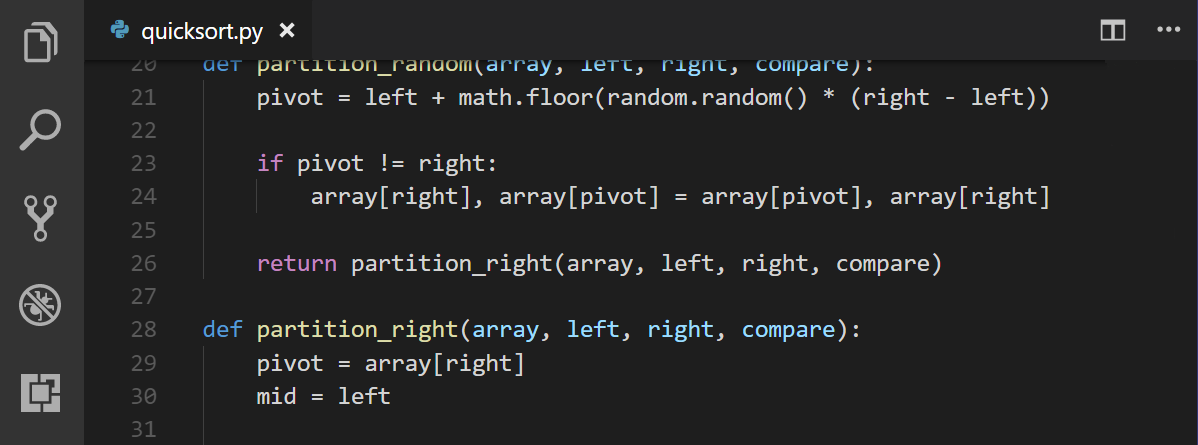
\includegraphics[width=1.0\textwidth]{Images/py_example.png}
	\caption{Пример типового листинга на языке Python в Visual Studio Code}
\end{figure}

Данный язык программирования поддерживает несколько парадигм программирования, в том числе структурное, объектно-ориентированное, функциональное и т.д. Основные черты - динамическая типизация, автоматическое управление памятью, поддержка многопоточных вычислений и многое другое. Важной особенностью является то, что не следует смешивать в листингах с кодом табуляцию и отступы с помощью пробелов, иначе это может привести к непредвиденным ошибкам.
\end{frame}
%%%%%%%%%%%%%%%%%%%%%%%%%%%%%%%%%%%%%%%%%%%%%%%%%%%%%%%%%%%%%%%%%
%%%%%%%%%%%%%%%%%%%%%%%%%%%%%%%%%%%%%%%%%%%%%%%%%%%%%%%%%%%%%%%%%
\begin{frame}{Установка Python}
Загрузить установочный файл \textit{Python} необходимой версии можно на официальном ресурсе \textit{https://www.python.org/downloads/}. Существует ряд библиотек, которые работают с \textit{Python} 2.7, не работают с \textit{Python} 3 и наоборот. Это связано с тем, что данные версии имеют между собой значительные различия, связанные не только с различным способом вызова \textit{print}, но и прочими, более глубокими структурными изменениями. В ходе установки крайне рекомендуется поставить флаг ADD TO PATH, что добавит переменную в переменные среды и предоставит доступ к Python из терминала. Чтобы проверить, установлен ли корректно \textit{Python} на ПК и узнать его версию, открываем терминал в Windows и вводим следующую команду:
\begin{figure}
	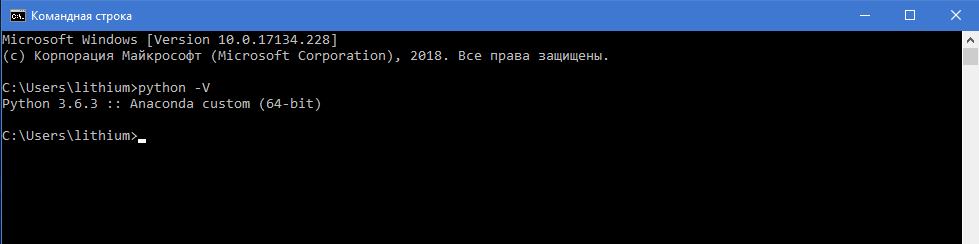
\includegraphics[width=1.0\textwidth]{Images/cmd.png}
	%\caption{Пример типового листинга на языке Python в Visual Studio Code}
\end{figure}
В случае успешной установки будет выведена вся необходимая информация. Если на компьютере установлено несколько версий \textit{Python}, то в команде может быть \textit{python3} или что-то аналогичное.


\end{frame}
%%%%%%%%%%%%%%%%%%%%%%%%%%%%%%%%%%%%%%%%%%%%%%%%%%%%%%%%%%%%%%%%%
%%%%%%%%%%%%%%%%%%%%%%%%%%%%%%%%%%%%%%%%%%%%%%%%%%%%%%%%%%%%%%%%%
\begin{frame}{Установка Anaconda}
Для того, чтобы использовать Python эффективнее и иметь множество заранее установленных базовых библиотек и сопутствующее им ПО, стоит установить бесплатный пакет Anaconda. Актуальную версию можно загрузить по официальному адресу \textit{https://www.anaconda.com/download/} для Python 2.7 или Python 3 соответственно. Также необходимо в ходе установки выбрать параметр Add to PATH.
\begin{figure}
	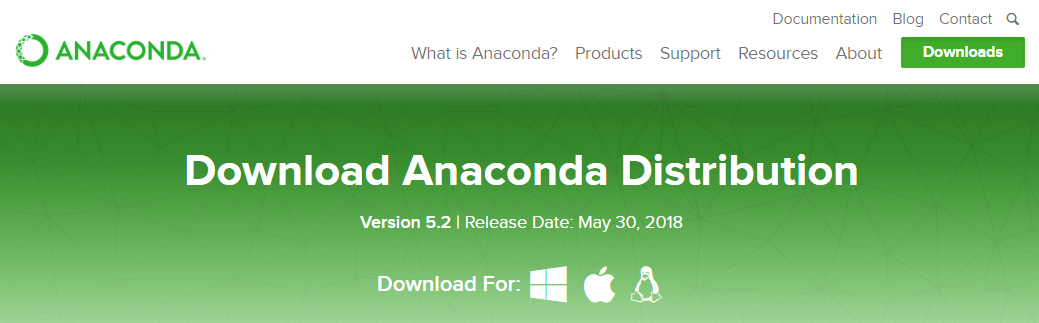
\includegraphics[width=1.0\textwidth]{Images/anac.png}
	%\caption{Пример типового листинга на языке Python в Visual Studio Code}
\end{figure}


\end{frame}
%%%%%%%%%%%%%%%%%%%%%%%%%%%%%%%%%%%%%%%%%%%%%%%%%%%%%%%%%%%%%%%%%
%%%%%%%%%%%%%%%%%%%%%%%%%%%%%%%%%%%%%%%%%%%%%%%%%%%%%%%%%%%%%%%%%
\begin{frame}{Синтаксис Python}


\begin{figure}
	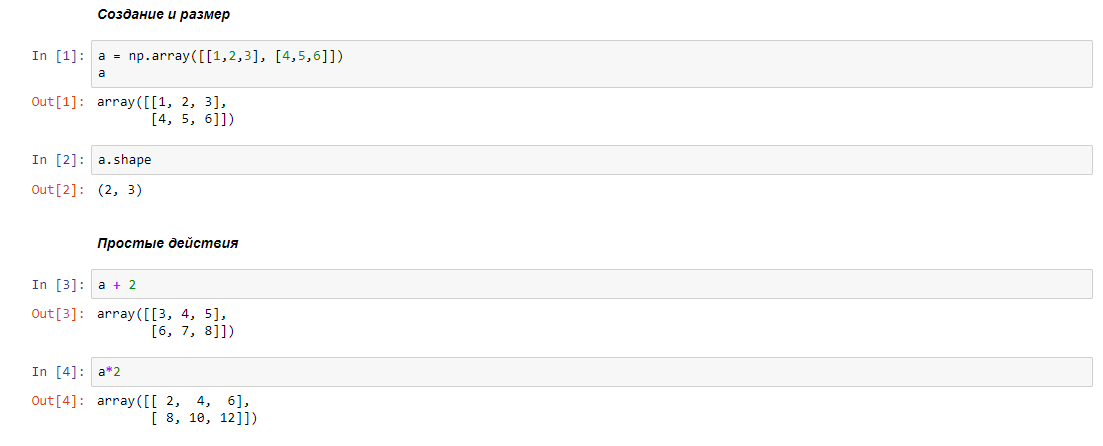
\includegraphics[width=1.0\textwidth]{Images/main1.png}
	%\caption{Пример типового листинга на языке Python в Visual Studio Code}
\end{figure}


\end{frame}
%%%%%%%%%%%%%%%%%%%%%%%%%%%%%%%%%%%%%%%%%%%%%%%%%%%%%%%%%%%%%%%%%
%%%%%%%%%%%%%%%%%%%%%%%%%%%%%%%%%%%%%%%%%%%%%%%%%%%%%%%%%%%%%%%%%
\begin{frame}{}


\begin{figure}
	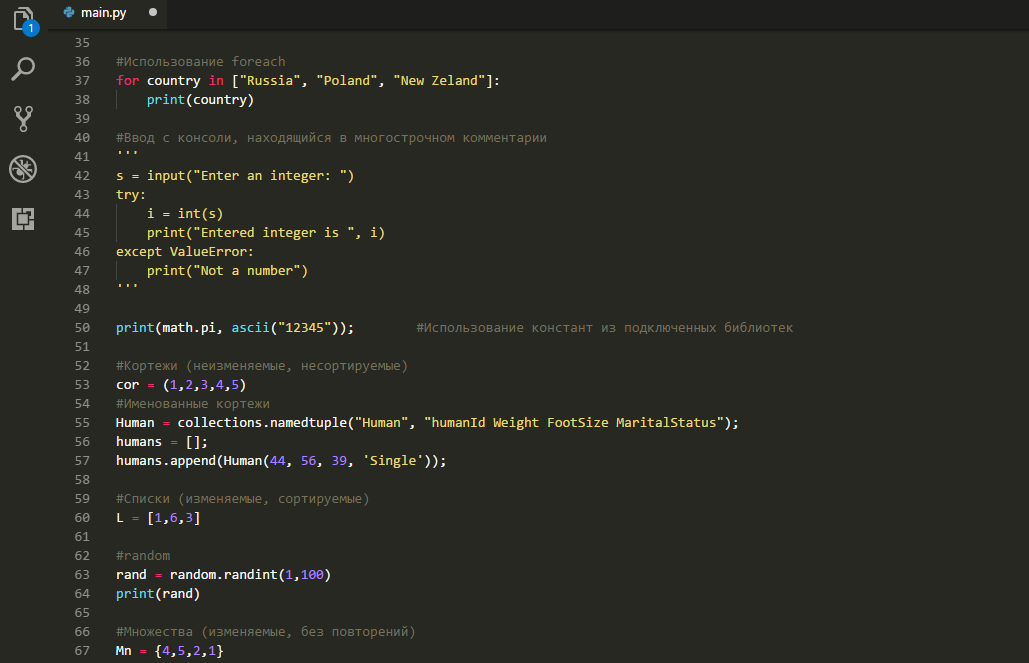
\includegraphics[width=1.0\textwidth]{Images/main2.png}
	%\caption{Пример типового листинга на языке Python в Visual Studio Code}
\end{figure}


\end{frame}
%%%%%%%%%%%%%%%%%%%%%%%%%%%%%%%%%%%%%%%%%%%%%%%%%%%%%%%%%%%%%%%%%
%%%%%%%%%%%%%%%%%%%%%%%%%%%%%%%%%%%%%%%%%%%%%%%%%%%%%%%%%%%%%%%%%
\begin{frame}{}


\begin{figure}
	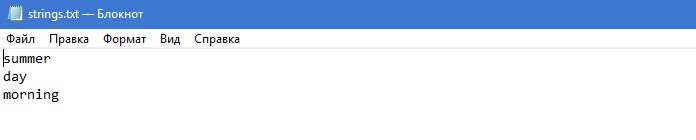
\includegraphics[width=1.0\textwidth]{Images/strings.png}
	%\caption{Пример типового листинга на языке Python в Visual Studio Code}
\end{figure}

\begin{figure}
	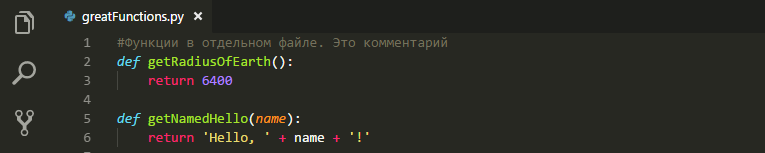
\includegraphics[width=1.0\textwidth]{Images/great.png}
	%\caption{Пример типового листинга на языке Python в Visual Studio Code}
\end{figure}


\end{frame}
%%%%%%%%%%%%%%%%%%%%%%%%%%%%%%%%%%%%%%%%%%%%%%%%%%%%%%%%%%%%%%%%%
%%%%%%%%%%%%%%%%%%%%%%%%%%%%%%%%%%%%%%%%%%%%%%%%%%%%%%%%%%%%%%%%%
\begin{frame}{}


\begin{figure}
	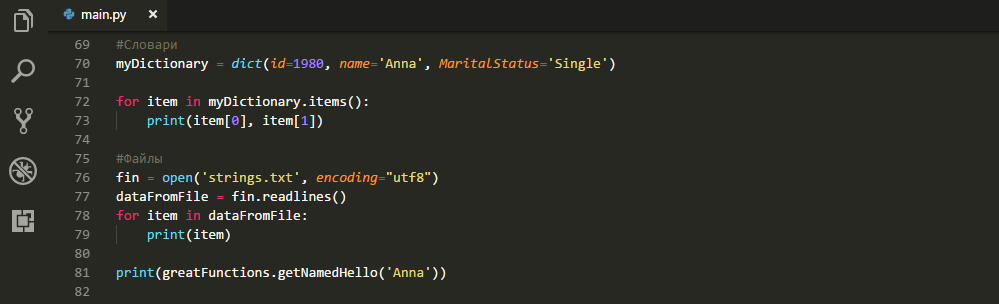
\includegraphics[width=1.0\textwidth]{Images/main3.png}
	%\caption{Пример типового листинга на языке Python в Visual Studio Code}
\end{figure}

\begin{figure}
	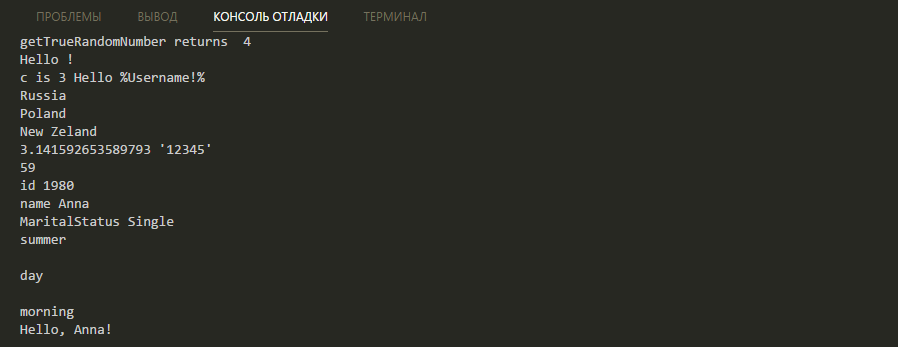
\includegraphics[width=1.0\textwidth]{Images/result.png}
	%\caption{Пример типового листинга на языке Python в Visual Studio Code}
\end{figure}



\end{frame}
%%%%%%%%%%%%%%%%%%%%%%%%%%%%%%%%%%%%%%%%%%%%%%%%%%%%%%%%%%%%%%%%%
%%%%%%%%%%%%%%%%%%%%%%%%%%%%%%%%%%%%%%%%%%%%%%%%%%%%%%%%%%%%%%%%%
\begin{frame}{Задания для практической работы}
\begin{figure}
	
\includegraphics[width=1.0\textwidth]{Images/codingtime.jpg}
	%\caption{Пример типового листинга на языке Python в Visual Studio Code}
\end{figure}
\begin{enumerate}
	\item Написать на Python рекурсивную функцию для получения $ 17 $ элемента ряда  Фибоначчи (каждое последующее число равно сумме двух предыдущих).
	\item Написать на Python рекурсивную функцию получения факториала числа $8$.
	\item Разделить полученное в пункте $ 2 $ на полученное в пункте $ 1 $ и умножить на значение числа Пи, взятое в пакете \textit{math}.
\end{enumerate}

\end{frame}
%%%%%%%%%%%%%%%%%%%%%%%%%%%%%%%%%%%%%%%%%%%%%%%%%%%%%%%%%%%%%%%%%
%%%%%%%%%%%%%%%%%%%%%%%%%%%%%%%%%%%%%%%%%%%%%%%%%%%%%%%%%%%%%%%%%
\begin{frame}{Решение задач}
\begin{figure}
	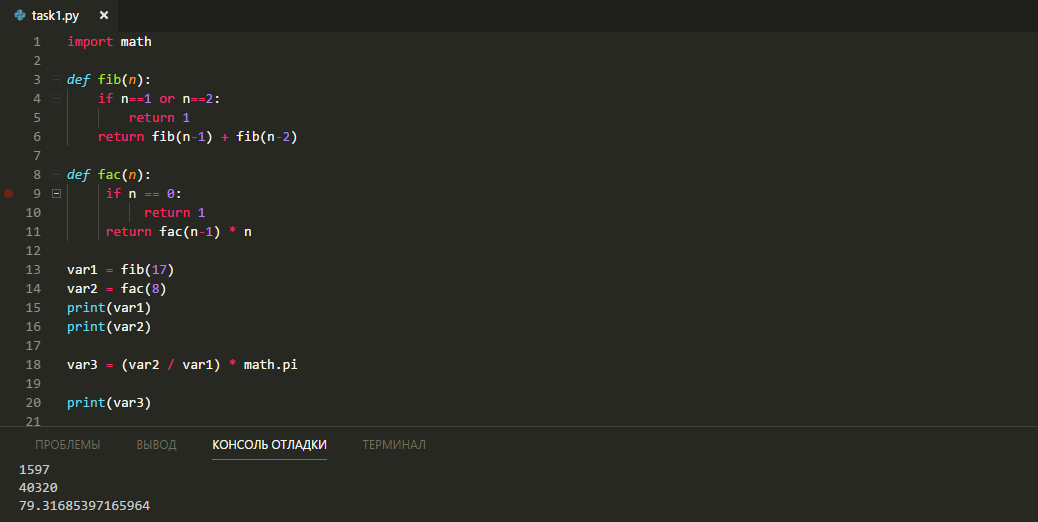
\includegraphics[width=1.0\textwidth]{Images/task1.PNG}
	%\caption{Пример типового листинга на языке Python в Visual Studio Code}
\end{figure}


\end{frame}
%%%%%%%%%%%%%%%%%%%%%%%%%%%%%%%%%%%%%%%%%%%%%%%%%%%%%%%%%%%%%%%%%
























%%%%%%%%%%%%%%%%%%%%%%%%%%%%%%%%%%%%%%%%%%%%%%%%%%%%%%%%%%%%%%%%%
%\begin{frame}{Blocks}
%
%\begin{block}{Block}
%Some examples of commonly used commands and features are included, to help you get started.
%\end{block}
%
%\begin{exampleblock}{Example Block}
%Some examples of commonly used commands and features are included, to help you get started.
%\end{exampleblock}
%
%\begin{alertblock}{Alert Block}
%Some examples of commonly used commands and features are included, to help you get started.
%\end{alertblock}
%
%\end{frame}












\end{document}